\chapter{Results and Discussion}
\label{chap:results}

This chapter reports software verification, analytical baselines,
Latin-hypercube exploration, multi-start optimization, finalist selection,
native CAD sweeps, CAD mass checks, and the bracket FEA quality-control
finding. Analytical, CAD, and FEA results are reported separately. The chapter
then answers the research questions and discusses the limitations of the
evidence.

\section{Verification Results}
\label{sec:software-results}

The offline verification campaign passed 27 tests; three Fusion-dependent
tests were excluded from that campaign because they require an active desktop
session. The completed checks covered the engineering definitions and bounds,
baseline feasibility, expected analytical trends, repeatable sampling,
bounded optimization, failed-evaluation containment, results recording, CAD
handoff, candidate preparation, and results review. Native-CAD sweeps were
evaluated separately in Section~\ref{sec:cad-sweep-results}; they did not
perform FEA.

\section{Analytical Optimization Results}
\label{sec:analytical-results}

\subsection{Baselines}
\label{sec:baseline-results}

\screeningwarning

Table~\ref{tab:baseline-results} gives the configured baselines. All three
passed the implemented factor-of-safety and displacement criteria.

\begin{table}[H]
\centering
\caption{Analytical baseline screening results}
\label{tab:baseline-results}
\resizebox{\textwidth}{!}{%
\begin{tabular}{lrrrrr}
\toprule
\textbf{Part} & \textbf{Mass (kg)} & \textbf{Stress (MPa)} &
\textbf{FOS} & \textbf{Deflection (mm)} & \textbf{Volume (m$^3$)}\\
\midrule
Bracket & 0.418125 & 41.5321 & 6.6455 & 0.195642 & 0.000154861\\
Padeye & 8.847625 & 46.1070 & 5.9644 & 0.013429 & 0.001127086\\
Stabilizer & 19.655593 & 86.9853 & 3.1730 & 3.336750 & 0.007279849\\
\bottomrule
\end{tabular}%
}
\end{table}

The bracket and padeye baselines had large yield-based margins. Their
deflection estimates were also well below the project limits. The stabilizer
had less factor-of-safety and displacement margin, although it remained
analytically feasible. These differences affected the available mass
reduction. A highly conservative baseline provides more room for a mass-only
optimizer than a baseline already close to an active constraint.

\subsection{Latin-Hypercube Exploration}
\label{sec:lhs-results}

Each part used 60 samples with seed 42. Table~\ref{tab:lhs-results} summarizes
the feasible counts and lightest feasible sampled designs.

\begin{table}[H]
\centering
\caption{Seeded Latin-hypercube results}
\label{tab:lhs-results}
\begin{tabularx}{\textwidth}{Xrrrr}
\toprule
\textbf{Part} & \textbf{Feasible samples} &
\textbf{Lightest mass (kg)} & \textbf{FOS} &
\textbf{Deflection (mm)}\\
\midrule
Bracket & 55 of 60 & 0.245687 & 10.4945 & 0.073331\\
Padeye & 60 of 60 & 5.923561 & 4.9324 & 0.010449\\
Stabilizer & 47 of 60 & 16.482802 & 2.7674 & 4.107580\\
\bottomrule
\end{tabularx}
\end{table}

The sample stage achieved its three intended purposes. It exercised broad
combinations of bounded variables, identified feasible low-mass starting
points, and showed that the parts had different constraint activity.

The bracket had five infeasible sampled designs, but its lightest feasible
sample still had high factor-of-safety margin. This indicates that broad
random combinations did not automatically exploit the dimensions that control
the screening stress.

All padeye samples were feasible. The result indicates that the declared
bounds and simplified stress model produce a generous feasible region under
the single project load case. It does not prove that every bounded padeye
would pass pin contact, weld, fatigue, or governing lifting rules.

The stabilizer had 13 infeasible samples. Its lightest feasible sample was
already close to both constraints compared with the other parts. The
stabilizer therefore presented the clearest constrained search.

\subsection{Multi-Start Optimization}
\label{sec:multistart-results}

Table~\ref{tab:multistart-results} gives the lightest feasible row found in
each local run. The start names identify the configured baseline and two
sample-derived starts.

\begin{table}[H]
\centering
\caption{Lightest feasible result from each Nelder--Mead start}
\label{tab:multistart-results}
\resizebox{\textwidth}{!}{%
\begin{tabular}{llrrrr}
\toprule
\textbf{Part} & \textbf{Start} & \textbf{Evaluations} &
\textbf{Mass (kg)} & \textbf{FOS} & \textbf{Deflection (mm)}\\
\midrule
\multirow{3}{*}{Bracket}
& Baseline & 132 & 0.126545 & 2.5530 & 0.475840\\
& Sample 1 & 126 & 0.116928 & 2.5208 & 0.396650\\
& Sample 2 & 129 & 0.113396 & 2.5386 & 0.369832\\
\midrule
\multirow{3}{*}{Padeye}
& Baseline & 108 & 3.837083 & 2.8528 & 0.026150\\
& Sample 1 & 116 & 3.609310 & 2.5767 & 0.026789\\
& Sample 2 & 109 & 3.547772 & 2.6224 & 0.027933\\
\midrule
\multirow{3}{*}{Stabilizer}
& Baseline & 110 & 14.414066 & 2.5041 & 3.932243\\
& Sample 1 & 116 & 14.315361 & 2.5149 & 3.822300\\
& Sample 2 & 111 & 14.391670 & 2.5331 & 3.847508\\
\bottomrule
\end{tabular}%
}
\end{table}

Every part benefited from more than one start. The lightest bracket and
padeye feasible designs came from the second sampled start. The lightest
stabilizer feasible design came from the first sampled start. If the study had
used only the configured baseline, the selected masses would have been higher
for all three parts.

The bracket baseline-start result approached the 0.5~mm displacement limit,
while the other two bracket results were governed more clearly by the
factor-of-safety limit. The padeye displacement remained far from 0.5~mm in
all runs, so its yield-based stress controlled the search. The stabilizer
operated close to the factor-of-safety limit while using approximately
76--79\% of the permitted displacement.

\subsection{Selected Finalists}
\label{sec:selected-finalists}

The validation packages selected the lightest explicitly feasible candidates.
Table~\ref{tab:selected-finalists} compares the selected finalist with its
baseline.

\begin{table}[H]
\centering
\caption{Selected analytical finalist compared with baseline}
\label{tab:selected-finalists}
\footnotesize
\begin{tabular*}{\textwidth}{@{\extracolsep{\fill}}lrrrrr}
\toprule
\textbf{Part} & \textbf{Baseline (kg)} &
\textbf{Finalist (kg)} & \textbf{Reduction} &
\textbf{Final FOS} & \textbf{Defl. (mm)}\\
\midrule
Bracket & 0.418125 & 0.113396 & 72.9\% & 2.5386 & 0.369832\\
Padeye & 8.847625 & 3.547772 & 59.9\% & 2.6224 & 0.027933\\
Stabilizer & 19.655593 & 14.315361 & 27.2\% & 2.5149 & 3.822300\\
\bottomrule
\end{tabular*}
\end{table}

\begin{figure}[H]
\centering
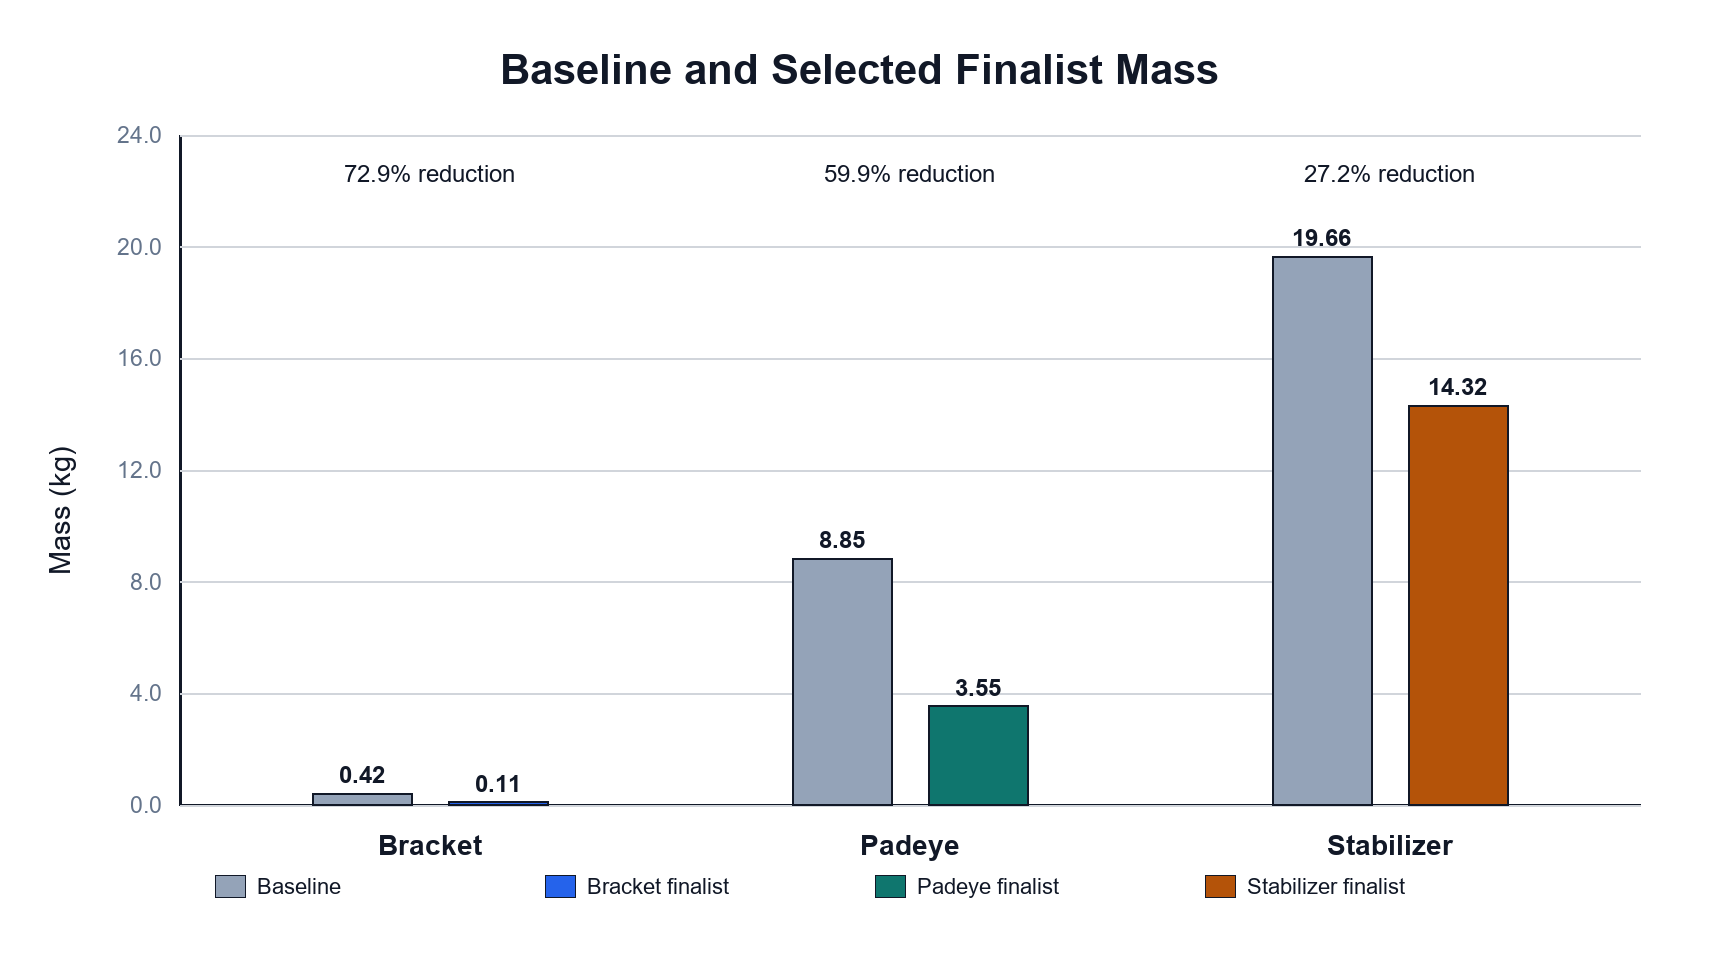
\includegraphics[width=\textwidth]{./images/charts/mass_baseline_finalist.png}
\caption{Analytical baseline and selected-finalist mass. Percentages are
screening reductions within the declared parameterized searches.}
\label{fig:mass-comparison}
\end{figure}

The reductions are large, particularly for the bracket and padeye. They must
be interpreted with the baseline and model scope. The baselines were
configured reference designs, not independently weight-optimized industrial
designs. The equations omit several failure modes. The percentage reduction
therefore measures the opportunity found by the implemented screening model,
not a validated service weight saving.

\subsection{Finalist Constraint Use}
\label{sec:constraint-use}

Figure~\ref{fig:constraint-use} normalizes the finalist responses. A
factor-of-safety ratio of 1.0 means the finalist is exactly at the minimum
factor of safety. A displacement ratio of 1.0 means it is exactly at the
displacement limit.

\begin{figure}[H]
\centering
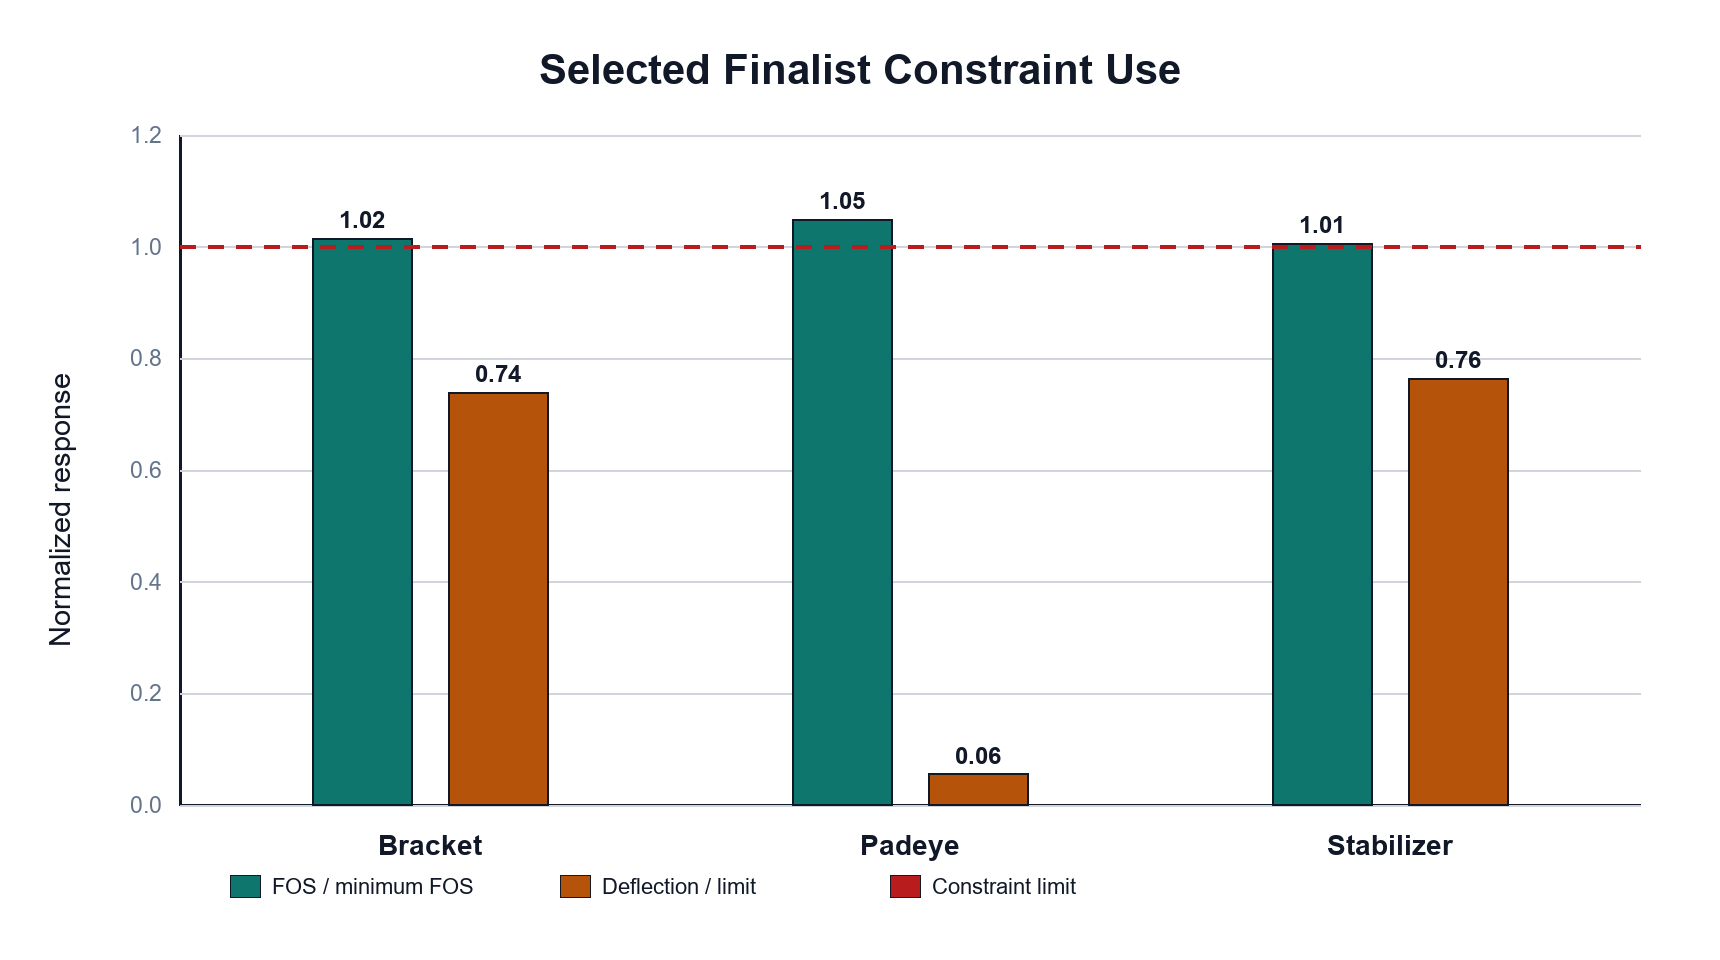
\includegraphics[width=\textwidth]{./images/charts/constraint_use.png}
\caption{Normalized constraint use for the selected analytical finalists}
\label{fig:constraint-use}
\end{figure}

All three finalists have factor-of-safety ratios only slightly above 1.0. This
result is expected from a mass-only search with a yield constraint: the
optimizer removes material until a constraint becomes active. The result also
shows why screening finalists need conservative backup candidates. A small
change in load, material, stress concentration, or model bias could make the
lightest row infeasible.

The bracket displacement ratio is approximately 0.74. The padeye displacement
ratio is approximately 0.056, so the simplified padeye search is almost
entirely controlled by stress. The stabilizer displacement ratio is
approximately 0.76. A later FEA model can change which constraint governs.

\subsection{Parameter Activity}
\label{sec:parameter-activity}

\subsubsection{Bracket}

The selected bracket used approximately 100.03~mm baseplate length,
80.94~mm width, 4.04~mm baseplate thickness, 33.26~mm rib height,
3.00~mm rib thickness, and 3.53~mm fillet radius. The length, width, plate
thickness, and rib thickness were near their lower bounds.

The pattern reflects the analytical equations. Plan dimensions and thickness
reduce volume directly. Rib height retains section depth and bending
resistance with less mass than a uniformly thick plate. This is a plausible
broad trend, but the candidate has little allowance for corrosion,
fabrication tolerance, weld size, bearing, or local plate action. The
lower-bound activity is therefore a prompt to review the bounds and omitted
constraints, not proof that the minimum gauge is suitable.

\subsubsection{Padeye}

The selected padeye used approximately 220.39~mm base length,
150.47~mm base width, 8.05~mm base thickness, 141.73~mm lug height,
12.16~mm lug thickness, 80.00~mm neck width, 70.00~mm gusset height,
6.21~mm gusset thickness, and 25.00~mm fillet radius.

Many thickness and envelope variables approached their lower bounds, while
the fillet radius reached its upper bound. In the analytical model, a large
fillet reduces the assumed concentration factor with a relatively modest
volume cost. The optimizer therefore spends material on the fillet while
reducing other dimensions. A three-dimensional contact and weld model may
change this balance.

\subsubsection{Stabilizer}

The selected stabilizer used approximately 4.01~mm skin, 25.0\% front-spar
position, 72.0\% rear-spar position, 7.85~mm front spar, 6.53~mm rear spar,
5.70~mm ribs, 221.48~mm root insert, 13.66~mm insert thickness, and
18.33~mm root fillet.

The skin approached its lower bound, while the spars moved apart. A larger spar
separation can increase effective section depth. The optimizer retained root
reinforcement to protect the factor-of-safety limit. This response is
consistent with the root-section model. It remains sensitive to the assumed
pressure distribution and omitted torsion and buckling.

\subsection{Penalty Objective and Explicit Feasibility}
\label{sec:penalty-results}

The smallest penalized objective in each stabilizer run was infeasible:

\begin{table}[H]
\centering
\caption{Infeasible minimum-objective rows from the stabilizer searches}
\label{tab:stabilizer-infeasible-objective}
\begin{tabularx}{\textwidth}{Xrrr}
\toprule
\textbf{Start} & \textbf{Objective} & \textbf{Mass (kg)} & \textbf{FOS}\\
\midrule
Baseline & 13.9702 & 13.74695 & 2.38188\\
Sample 1 & 13.7477 & 13.61934 & 2.41042\\
Sample 2 & 13.7335 & 13.61934 & 2.41554\\
\bottomrule
\end{tabularx}
\end{table}

The penalty increased the objective, but the low mass remained attractive
enough to produce a smaller value than the feasible rows. If the package had
selected the minimum objective without a feasibility filter, it would have
promoted a failed design. The implemented selection avoided this error.

This result shows a limitation and a strength. The fixed penalty weight is not
strong enough to make every run's objective minimum feasible. However, the
system does not treat the penalty as the acceptance rule. Explicit feasibility
is the acceptance rule. Future work can compare adaptive penalties,
feasibility-first ranking, or a constrained derivative-free method.

\section{CAD Verification Results}
\label{sec:cad-results}

\subsection{Native CAD Generator Sweeps}
\label{sec:cad-sweep-results}

The final sweeps used generator version 2.4. Table~\ref{tab:cad-sweep-results}
reports their status.

\begin{table}[H]
\centering
\caption{Baseline plus 20-vector native CAD sweep results}
\label{tab:cad-sweep-results}
\begin{tabularx}{\textwidth}{
    >{\raggedright\arraybackslash}X
    rr
    >{\raggedright\arraybackslash}X}
\toprule
\textbf{Part} & \textbf{Artifacts created} & \textbf{Integration passes} &
\textbf{Recorded observation}\\
\midrule
Bracket & 21 of 21 & 21 of 21 &
Completed in approximately 238.19~s.\\
Padeye & 21 of 21 & 21 of 21 &
Completed in approximately 157.19~s.\\
Stabilizer & 21 of 21 & Final read timed out &
All 21 artifacts were created. The outer test reached its 30-minute timeout
while reading the final response; direct artifact audit confirmed generation.\\
\bottomrule
\end{tabularx}
\end{table}

Every audited case contained one connected solid, positive volume, STEP
output, boundary metadata, and non-empty required boundary roles. The result
supports generator behavior over the seeded bounded vectors. It does not prove
behavior for every possible point in the continuous design space.

The stabilizer timeout is reported rather than hidden. The evidence supports
successful artifact generation for all 21 vectors, but it does not support a
claim that the complete outer integration test exited normally. The event
also shows why long-running desktop automation should preserve intermediate
artifacts and per-case records.

\subsection{Analytical and Native-CAD Mass Comparison}
\label{sec:cad-mass-results}

Table~\ref{tab:cad-mass-comparison} compares analytical and Fusion CAD mass
for each baseline and selected finalist. The percentage difference is
calculated relative to the analytical mass.

\begin{table}[H]
\centering
\caption{Analytical and native-CAD mass comparison}
\label{tab:cad-mass-comparison}
\begin{tabularx}{\textwidth}{XXrrr}
\toprule
\textbf{Part} & \textbf{Design} & \textbf{Analytical (kg)} &
\textbf{Fusion CAD (kg)} & \textbf{Difference}\\
\midrule
Bracket & Baseline & 0.418125 & 0.422813 & +1.12\%\\
Bracket & Finalist & 0.113396 & 0.114705 & +1.15\%\\
Padeye & Baseline & 8.847625 & 8.897275 & +0.56\%\\
Padeye & Finalist & 3.547772 & 3.682599 & +3.80\%\\
Stabilizer & Baseline & 19.655593 & 19.297290 & -1.82\%\\
Stabilizer & Finalist & 14.315361 & 14.400328 & +0.59\%\\
\bottomrule
\end{tabularx}
\end{table}

\begin{figure}[H]
\centering
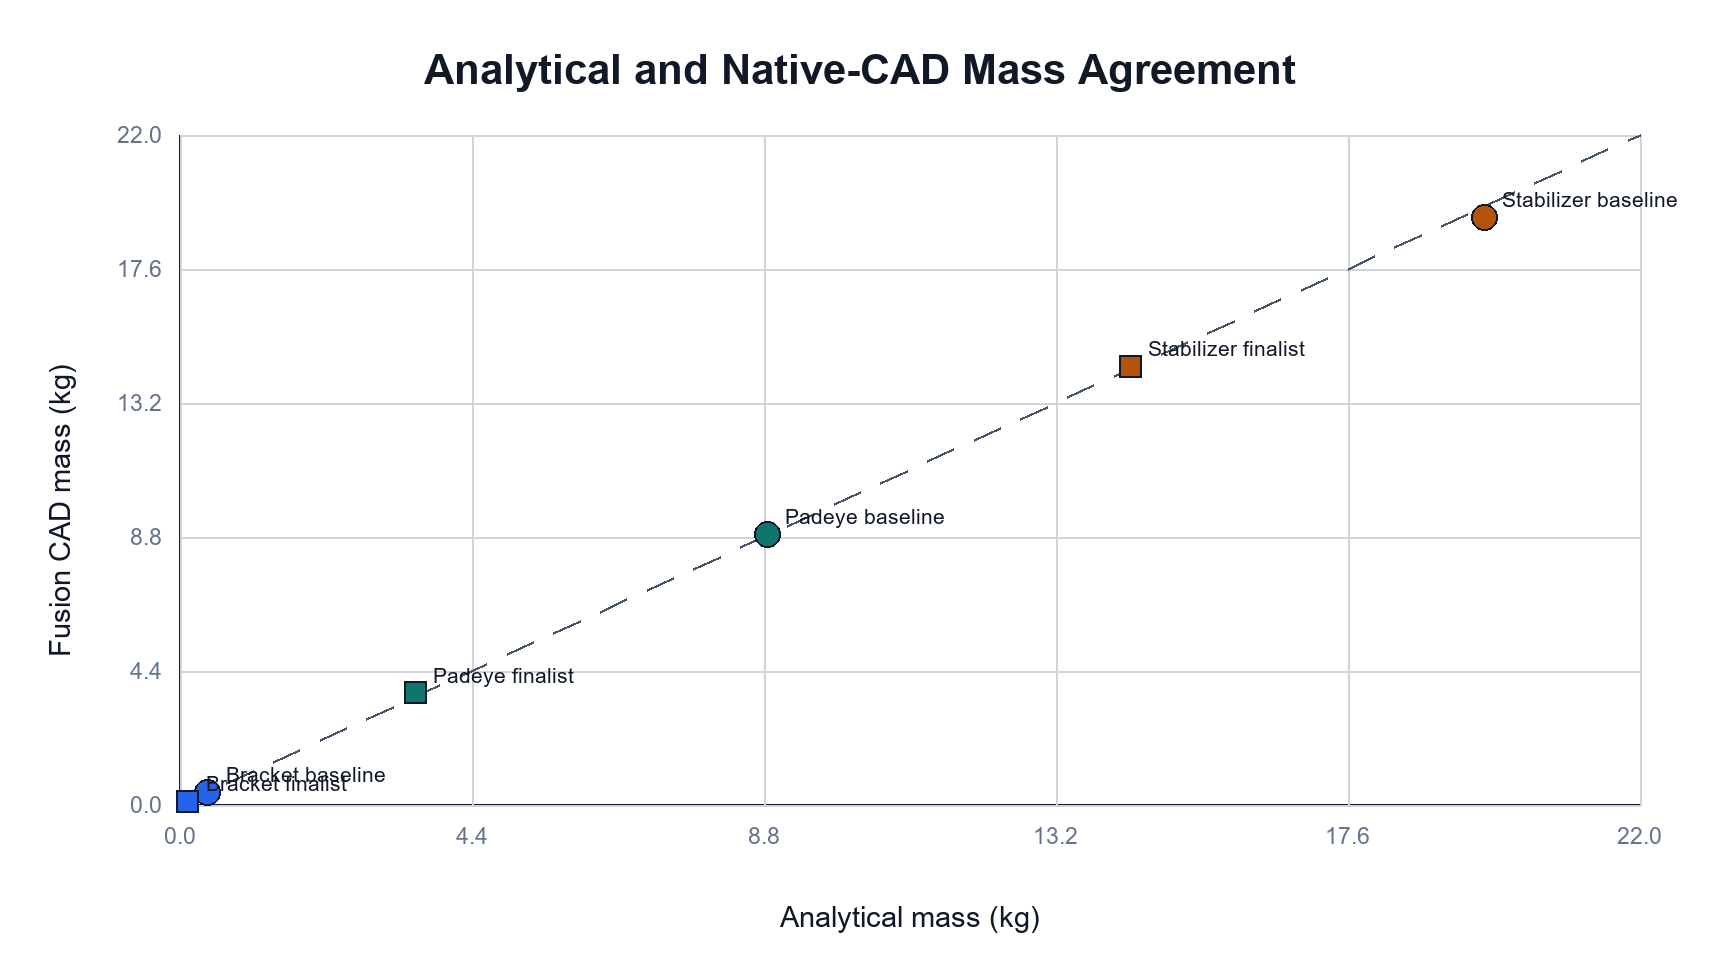
\includegraphics[width=0.86\textwidth]{./images/charts/cad_mass_agreement.png}
\caption{Analytical mass compared with Fusion native-CAD mass. The diagonal
shows exact agreement.}
\label{fig:cad-mass-agreement}
\end{figure}

All six differences were within 3.8\%. The agreement supports the broad
volume approximations used for mass ranking. The padeye finalist showed the
largest difference, which is consistent with greater geometric complexity
around the lug crown, fillets, and gusset intersections.

The agreement does not validate stress. Mass depends primarily on volume and
density. Structural response depends on the load path, section properties,
local geometry, support idealization, contact, and mesh. The CAD response
therefore remains correctly marked as partial.

\section{Bracket Static Stress Study Evidence}
\label{sec:bracket-fea-result}

Two bracket Static Stress reports were available for review. Study~1 records
the first exploratory solve, while Study~2 documents a revised setup with
explicit images of the constrained and loaded faces. Both studies use the
same bracket form and Aluminum 6061 material. Figure~\ref{fig:bracket-study-setups}
shows the progression from the generated geometry to the more clearly
documented boundary conditions.

\begin{figure}[H]
\centering
\begin{minipage}[t]{0.58\textwidth}
\centering
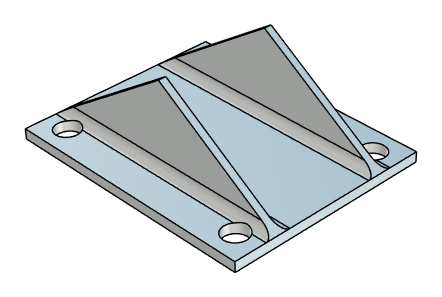
\includegraphics[width=\textwidth]{./images/fusion/study_1_02.png}
\caption*{(a) Study~1 bracket geometry}
\end{minipage}

\vspace{0.3cm}
\begin{minipage}[t]{0.48\textwidth}
\centering
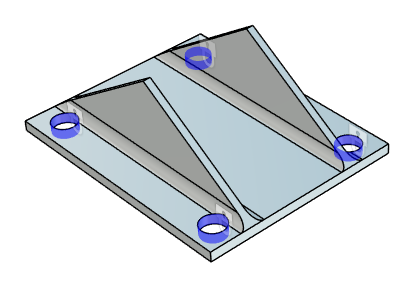
\includegraphics[width=\textwidth]{./images/fusion/study_2_03.png}
\caption*{(b) Study~2 mounting-hole constraints}
\end{minipage}
\hfill
\begin{minipage}[t]{0.48\textwidth}
\centering
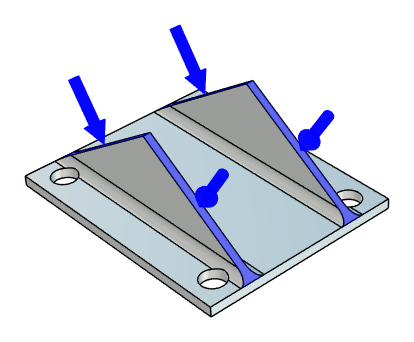
\includegraphics[width=\textwidth]{./images/fusion/study_2_04.png}
\caption*{(c) Study~2 rib-face loading}
\end{minipage}
\caption{Bracket geometry and boundary-condition evidence from the two Fusion
studies. Study~2 makes the four constrained mounting holes and four loaded
upper rib faces visible.}
\label{fig:bracket-study-setups}
\end{figure}

The support regions in Figure~\ref{fig:bracket-study-setups}(b) correspond to
the four cylindrical mounting-hole faces. This is a useful first
idealization of a rigid bolt-down, although it does not represent bolt
preload, clearance, bearing, or contact with the supporting structure. The
arrows in Figure~\ref{fig:bracket-study-setups}(c) confirm that the upper
sloping faces of both ribs were selected for loading. The Study~2 data,
however, record a total magnitude of 1.472~N with \emph{force per entity}
disabled. The intended total was 1472~N. The recorded force also contains both
$X$ and $Z$ components, which makes direction another item that must be
confirmed in the corrected study.

Table~\ref{tab:bracket-study-comparison} summarizes the numerical evidence.
Study~1 does not provide a complete applied-load record, but its reported
1.298~N support reaction and very small response show that it also operated at
a newton-scale load. Study~2 improves traceability but preserves the
factor-of-one-thousand magnitude error.

\begin{table}[H]
\centering
\caption{Comparison of the two exploratory bracket studies}
\label{tab:bracket-study-comparison}
\begin{tabularx}{\textwidth}{
    >{\raggedright\arraybackslash}p{0.25\textwidth}
    >{\raggedright\arraybackslash}X
    >{\raggedright\arraybackslash}X}
\toprule
\textbf{Recorded item} & \textbf{Study 1} & \textbf{Study 2}\\
\midrule
Load evidence &
No complete applied-load table; reported support reaction magnitude
1.298~N &
1.472~N total; force per entity disabled; $X=-0.815$~N and
$Z=-1.226$~N\\
\addlinespace[0.35em]
Mesh evidence &
Parabolic elements; 10\% average element size; no refinement step &
Parabolic elements; 4781 nodes and 2355 elements; 10\% average element
size; no refinement step\\
\addlinespace[0.35em]
Maximum von Mises stress &
0.016~MPa &
0.026~MPa\\
\addlinespace[0.35em]
Minimum factor of safety &
17\,628 &
10\,479\\
\addlinespace[0.35em]
Maximum displacement &
$4.595\times10^{-6}$~mm &
$9.223\times10^{-6}$~mm\\
\addlinespace[0.35em]
Engineering status &
Rejected because the loading is incomplete and inconsistent with the
1.4715~kN design envelope &
Rejected because 1.472~N was applied instead of 1472~N; direction and
reaction balance also require confirmation\\
\bottomrule
\end{tabularx}
\end{table}

The factor-of-safety plots in Figure~\ref{fig:bracket-fos-comparison} are
almost uniformly blue because the display is capped at 8 while the reported
minimum factors of safety exceed ten thousand. The images are therefore
evidence of an unrealistically lightly loaded model, not evidence of a highly
efficient bracket. They also illustrate why a colour plot must be read
together with its legend and input table.

\begin{figure}[H]
\centering
\begin{minipage}{0.88\textwidth}
\centering
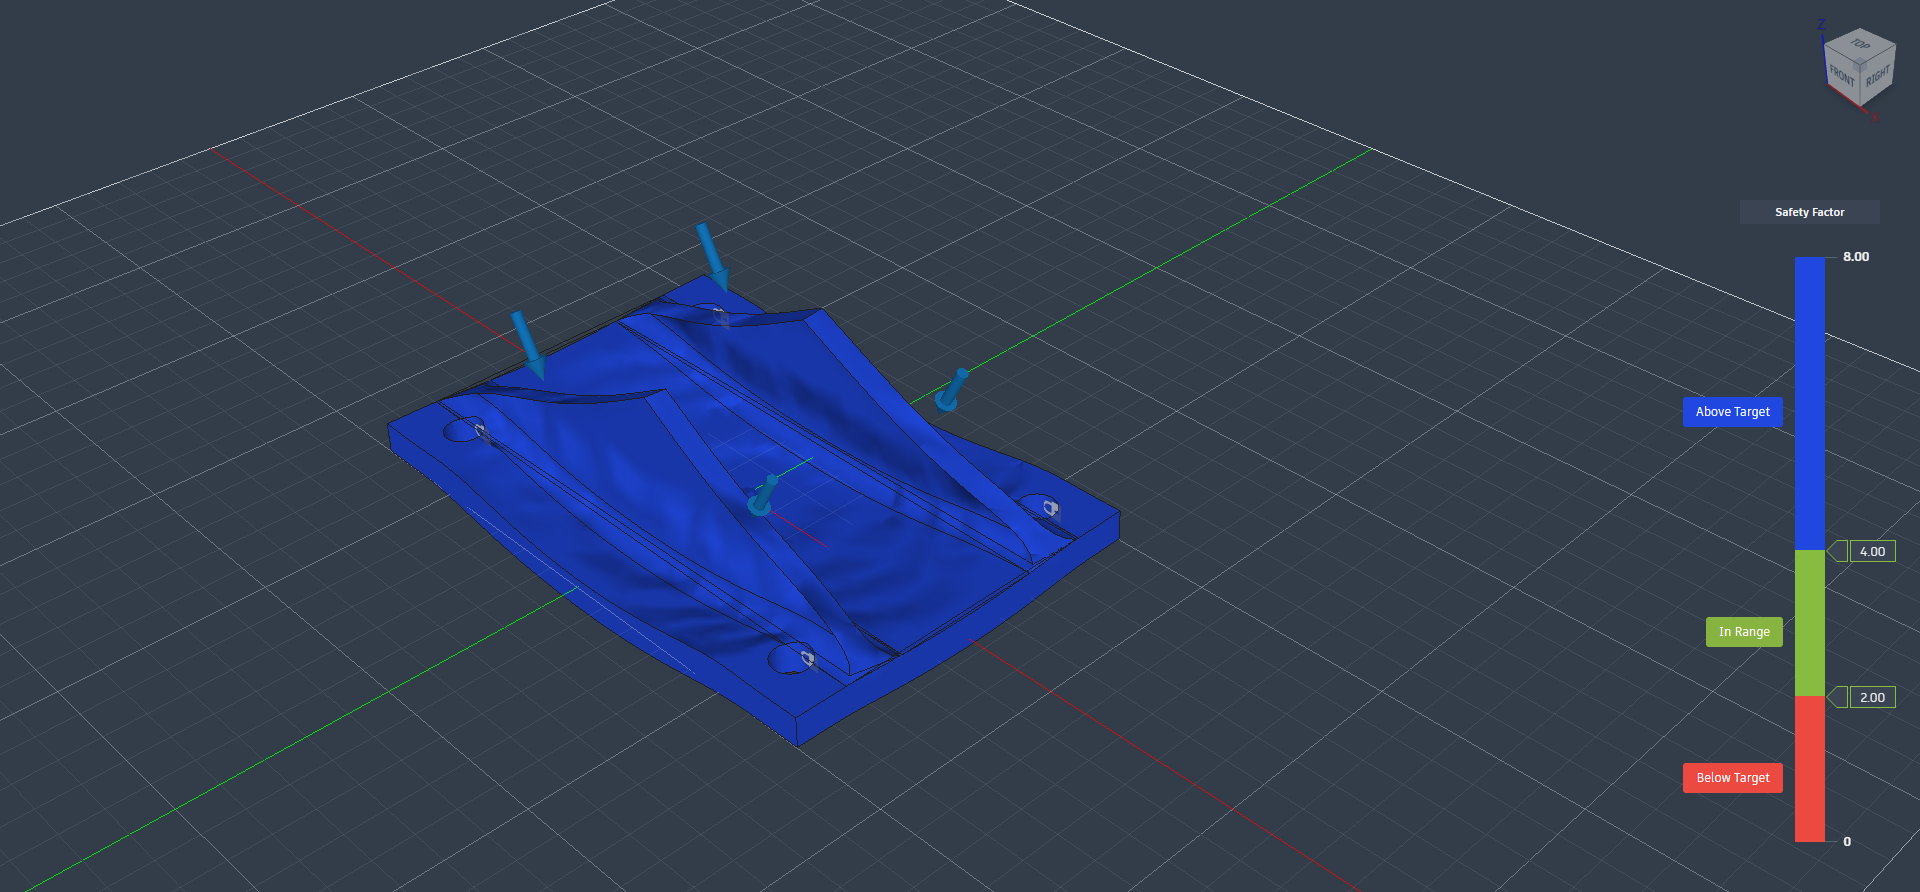
\includegraphics[width=\textwidth]{./images/fusion/study_1_03.png}
\caption*{(a) Study~1 factor-of-safety plot}
\end{minipage}

\vspace{0.25cm}
\begin{minipage}{0.88\textwidth}
\centering
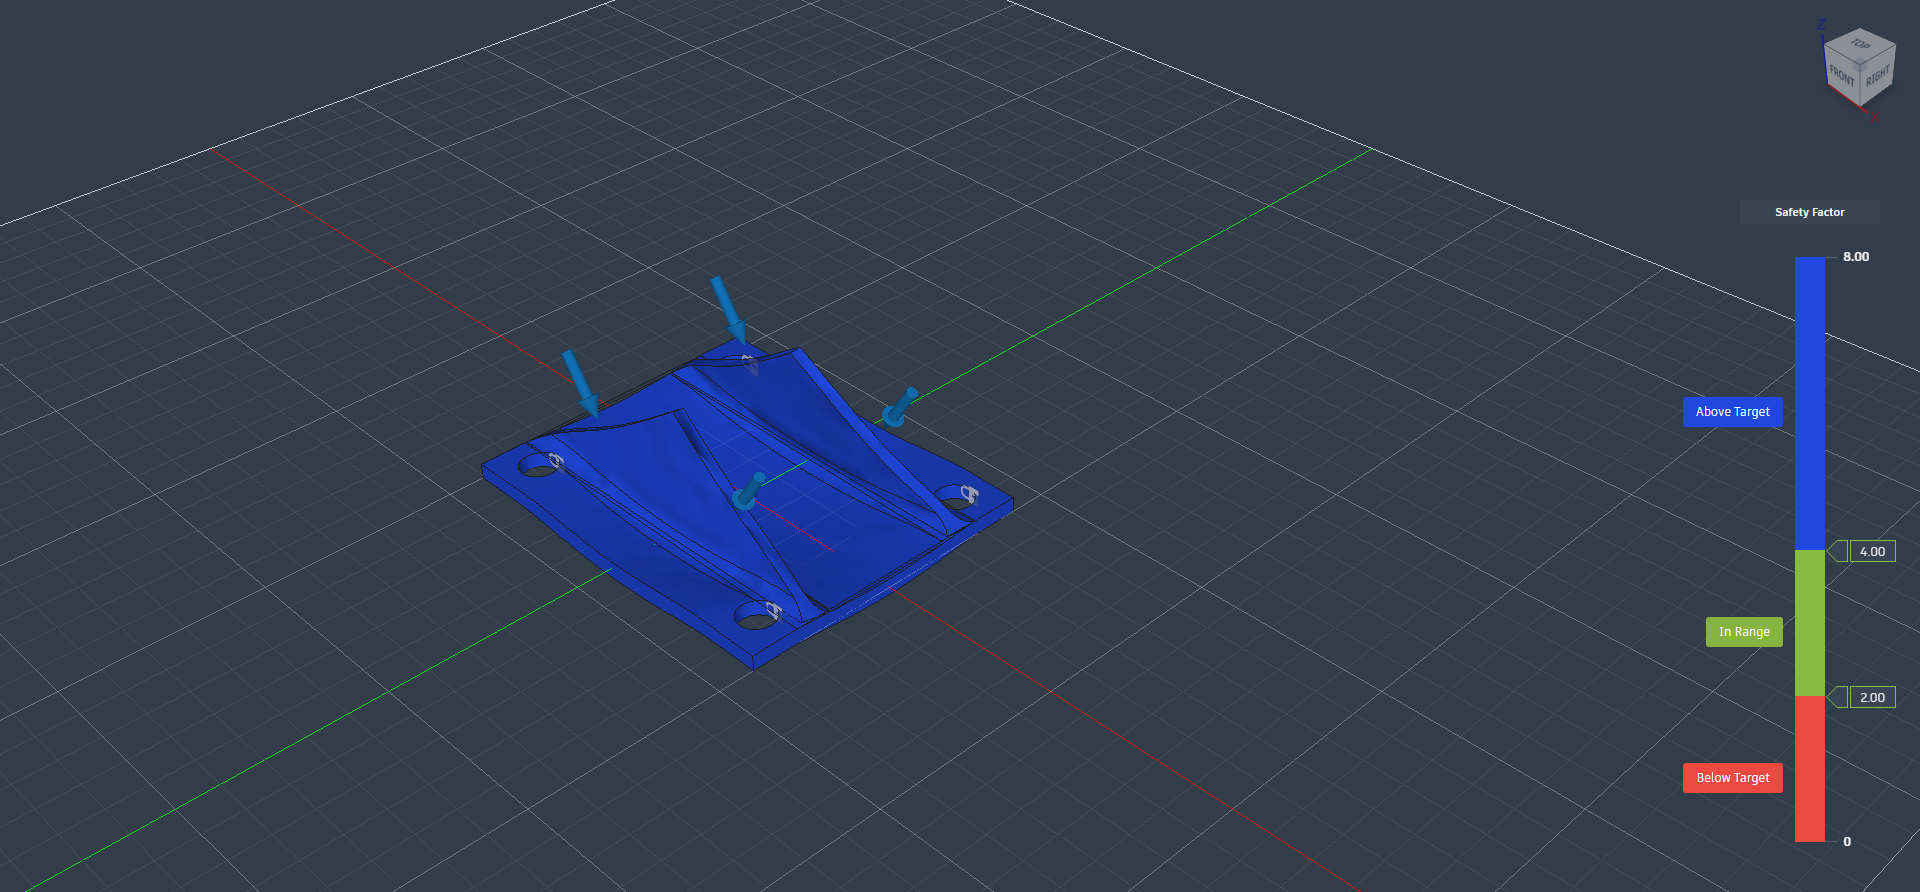
\includegraphics[width=\textwidth]{./images/fusion/study_2_05.png}
\caption*{(b) Study~2 factor-of-safety plot}
\end{minipage}
\caption{Factor-of-safety plots from Studies~1 and~2. The common display cap
of 8 masks the much larger reported values produced by the incorrect
newton-scale loading.}
\label{fig:bracket-fos-comparison}
\end{figure}

The von Mises plots in Figure~\ref{fig:bracket-stress-comparison} show higher
stress around the mounting-hole edges, rib roots, and load-introduction
regions. These locations are consistent with the expected load path and
identify where local mesh refinement and more realistic bolt/contact modelling
would be required. The maxima of 0.016~MPa and 0.026~MPa cannot be used for
acceptance because neither study represents the design load.

\begin{figure}[H]
\centering
\begin{minipage}{0.88\textwidth}
\centering
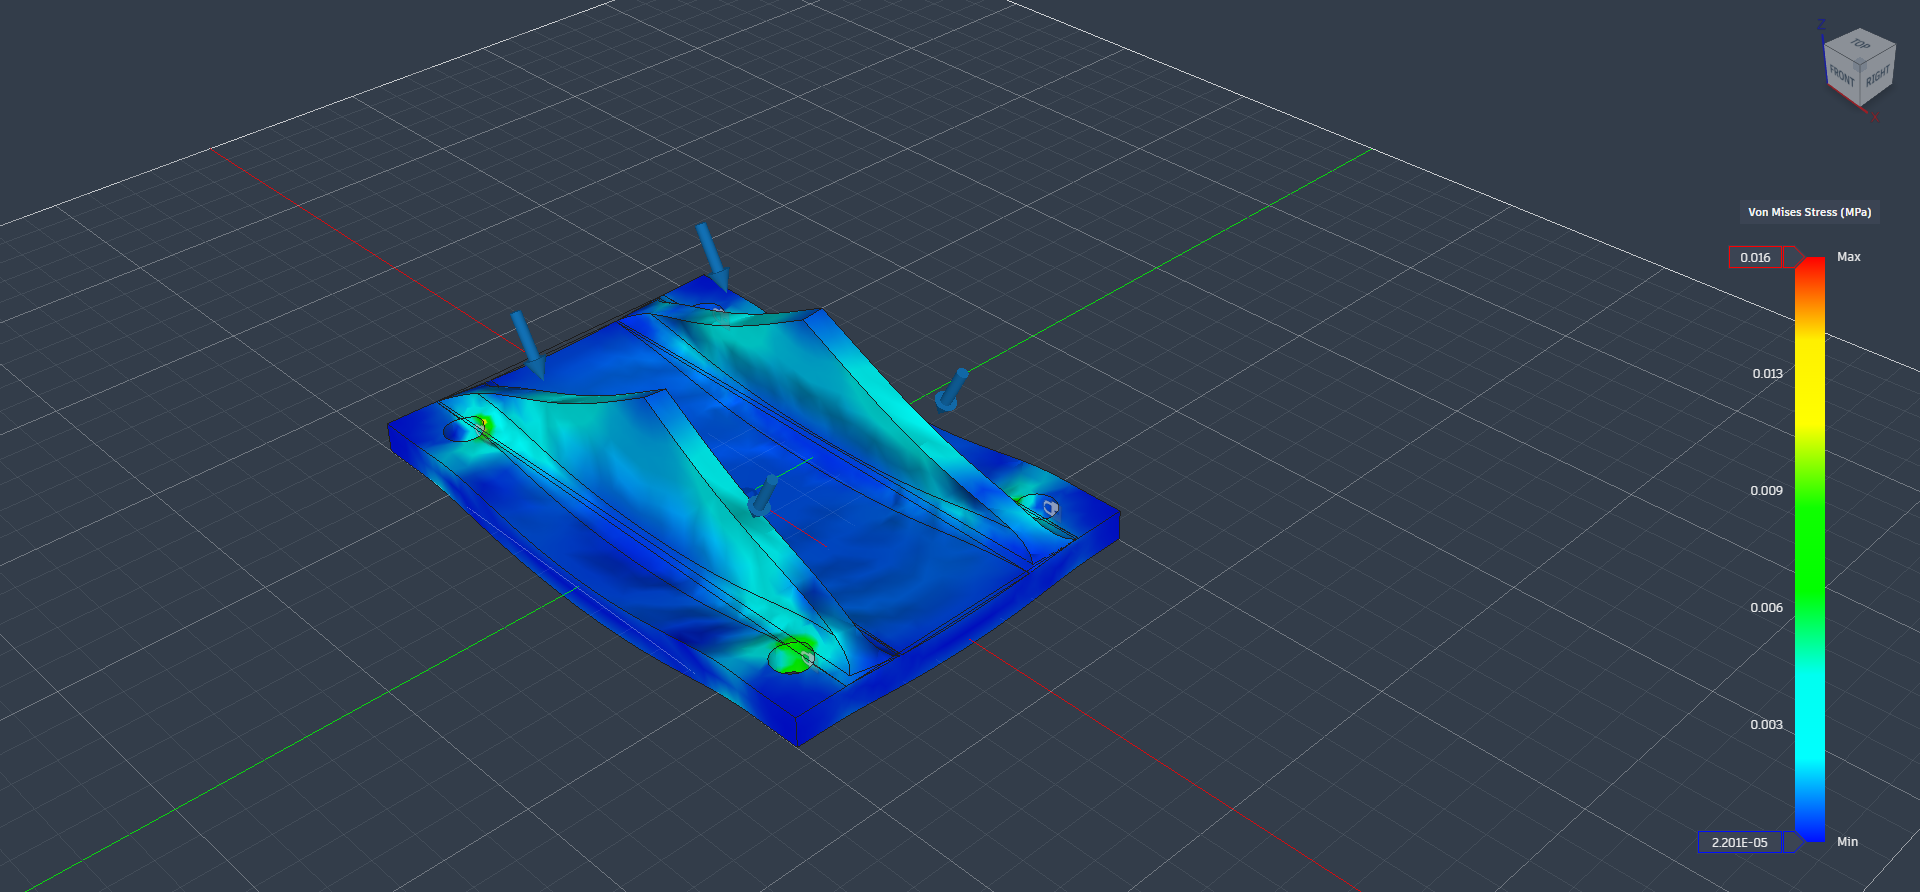
\includegraphics[width=\textwidth]{./images/fusion/study_1_05.png}
\caption*{(a) Study~1 von Mises stress}
\end{minipage}

\vspace{0.25cm}
\begin{minipage}{0.88\textwidth}
\centering
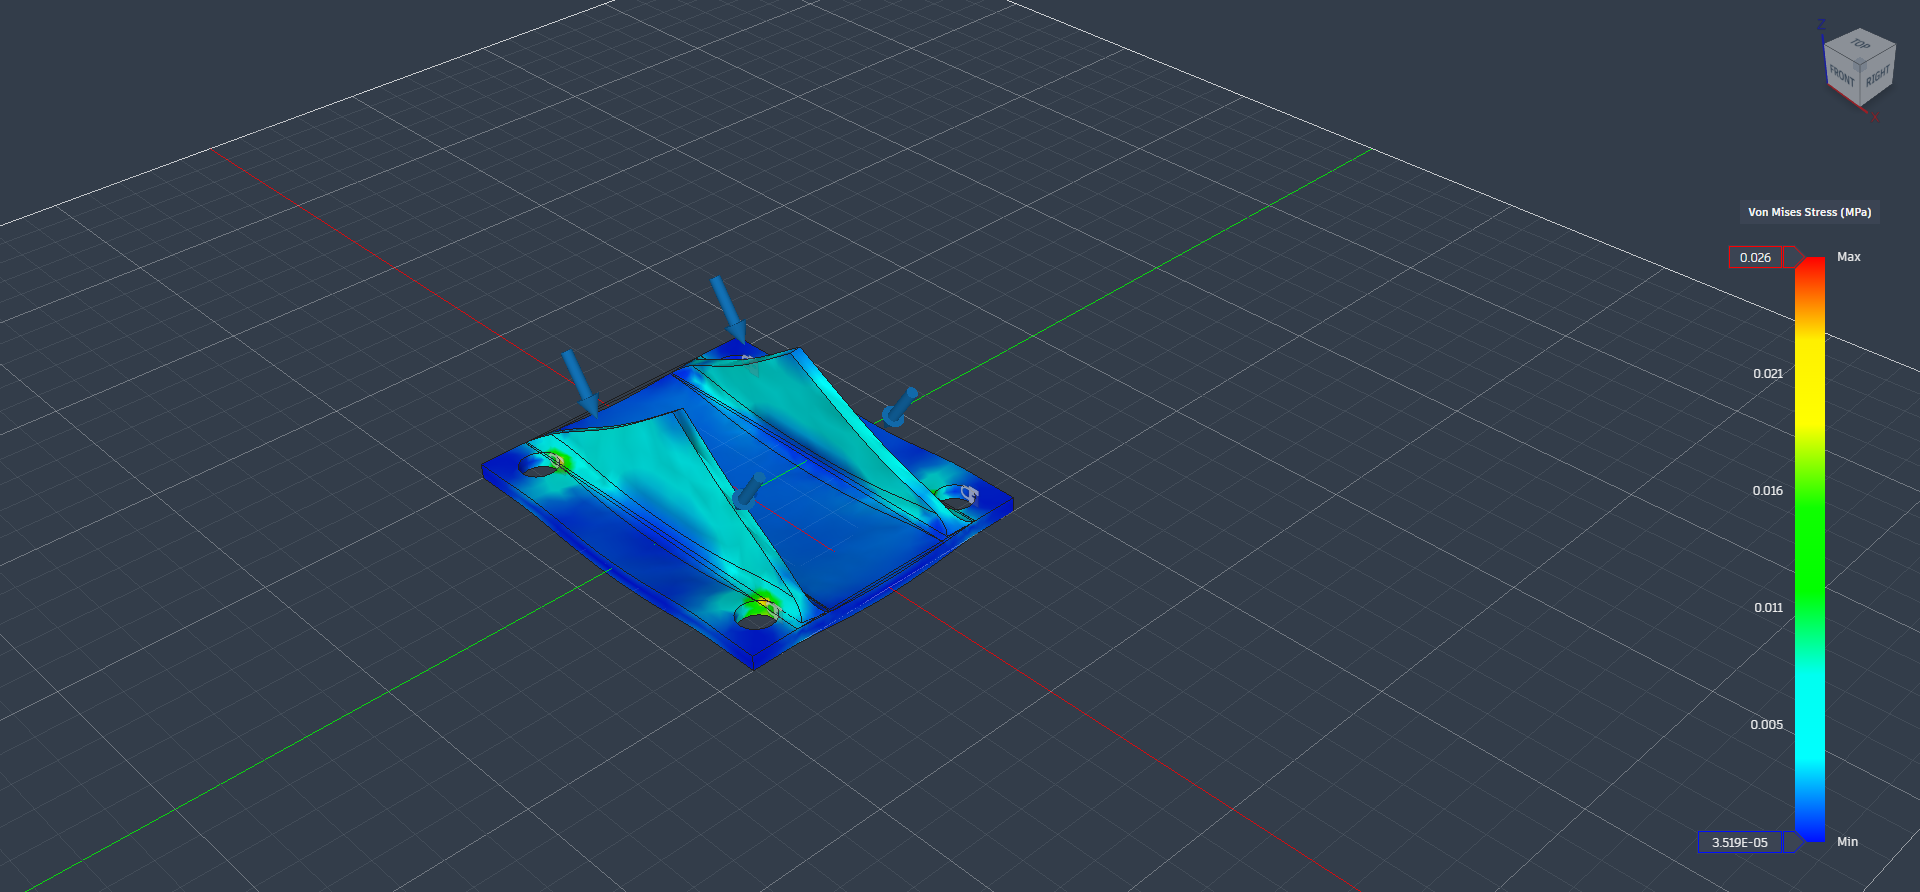
\includegraphics[width=\textwidth]{./images/fusion/study_2_07.png}
\caption*{(b) Study~2 von Mises stress}
\end{minipage}
\caption{Von Mises stress distributions from the two exploratory studies.
Only the qualitative locations are retained as useful evidence.}
\label{fig:bracket-stress-comparison}
\end{figure}

Figure~\ref{fig:bracket-displacement-comparison} shows minimum displacement
near the constrained mounting holes and larger movement across the
unconstrained plate and rib regions. This is qualitatively consistent with the
selected supports. The two maximum values remain several orders of magnitude
below the analytical screening displacement because the applied study loads
were several orders of magnitude too small. No calibration conclusion can
therefore be drawn from the apparent difference between the analytical and
solver responses.

\begin{figure}[H]
\centering
\begin{minipage}{0.88\textwidth}
\centering
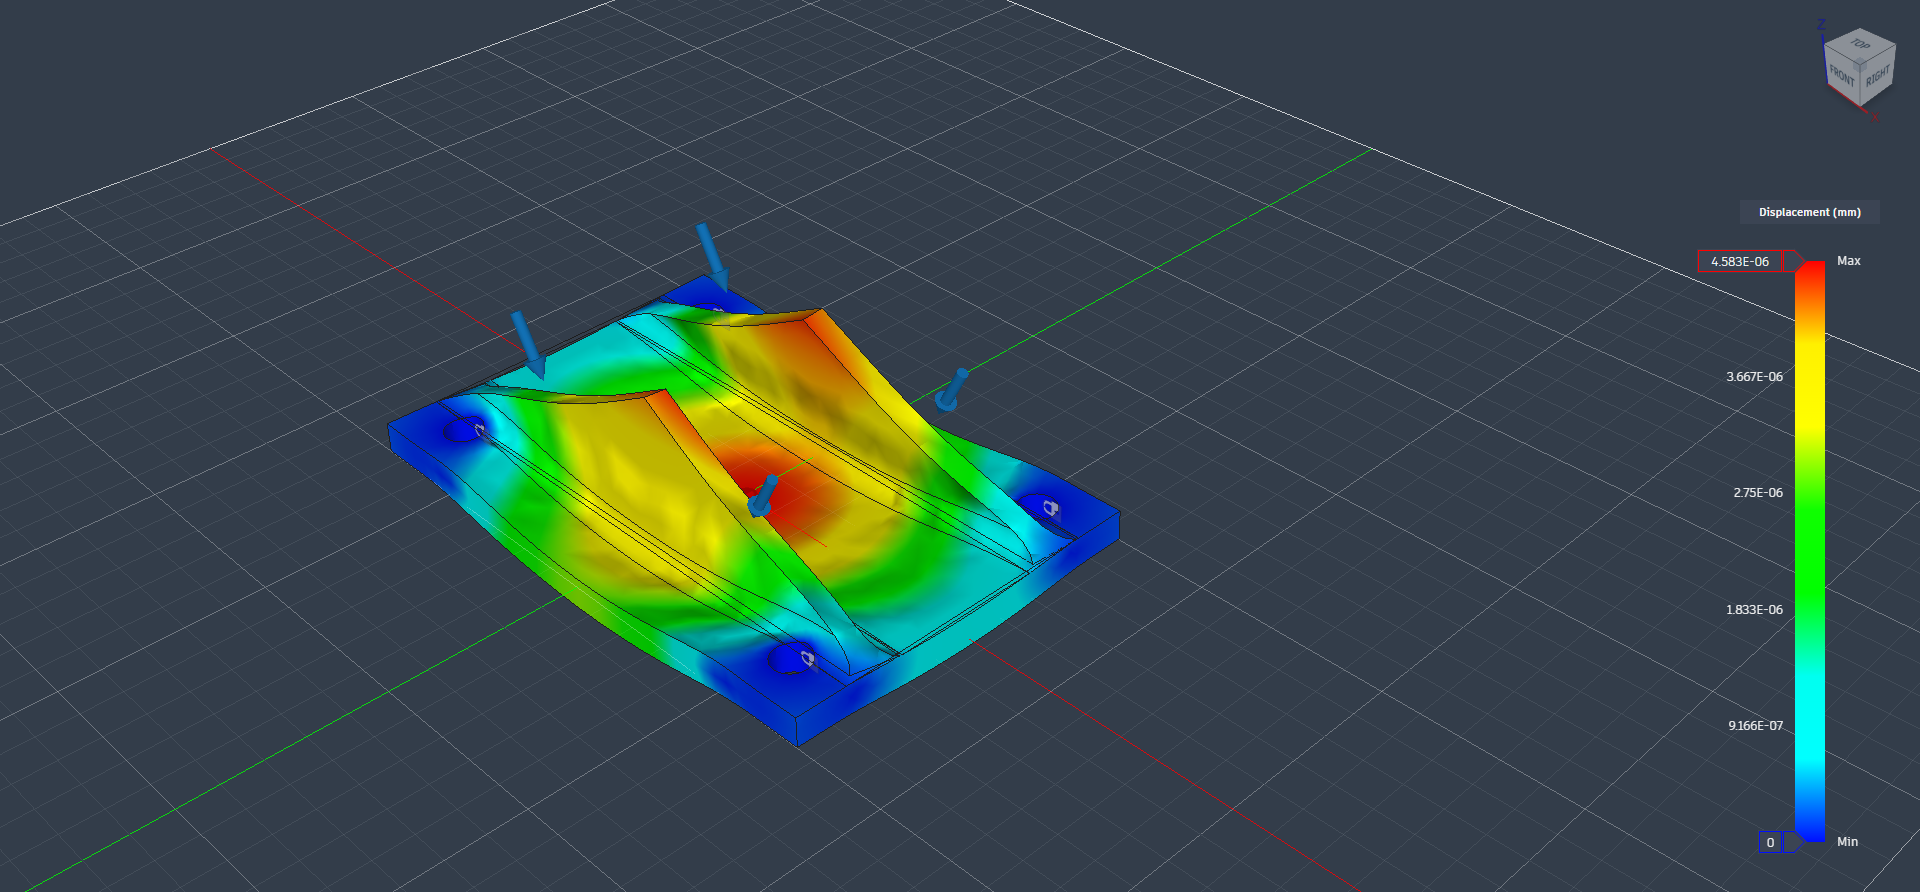
\includegraphics[width=\textwidth]{./images/fusion/study_1_08.png}
\caption*{(a) Study~1 total displacement}
\end{minipage}

\vspace{0.25cm}
\begin{minipage}{0.88\textwidth}
\centering
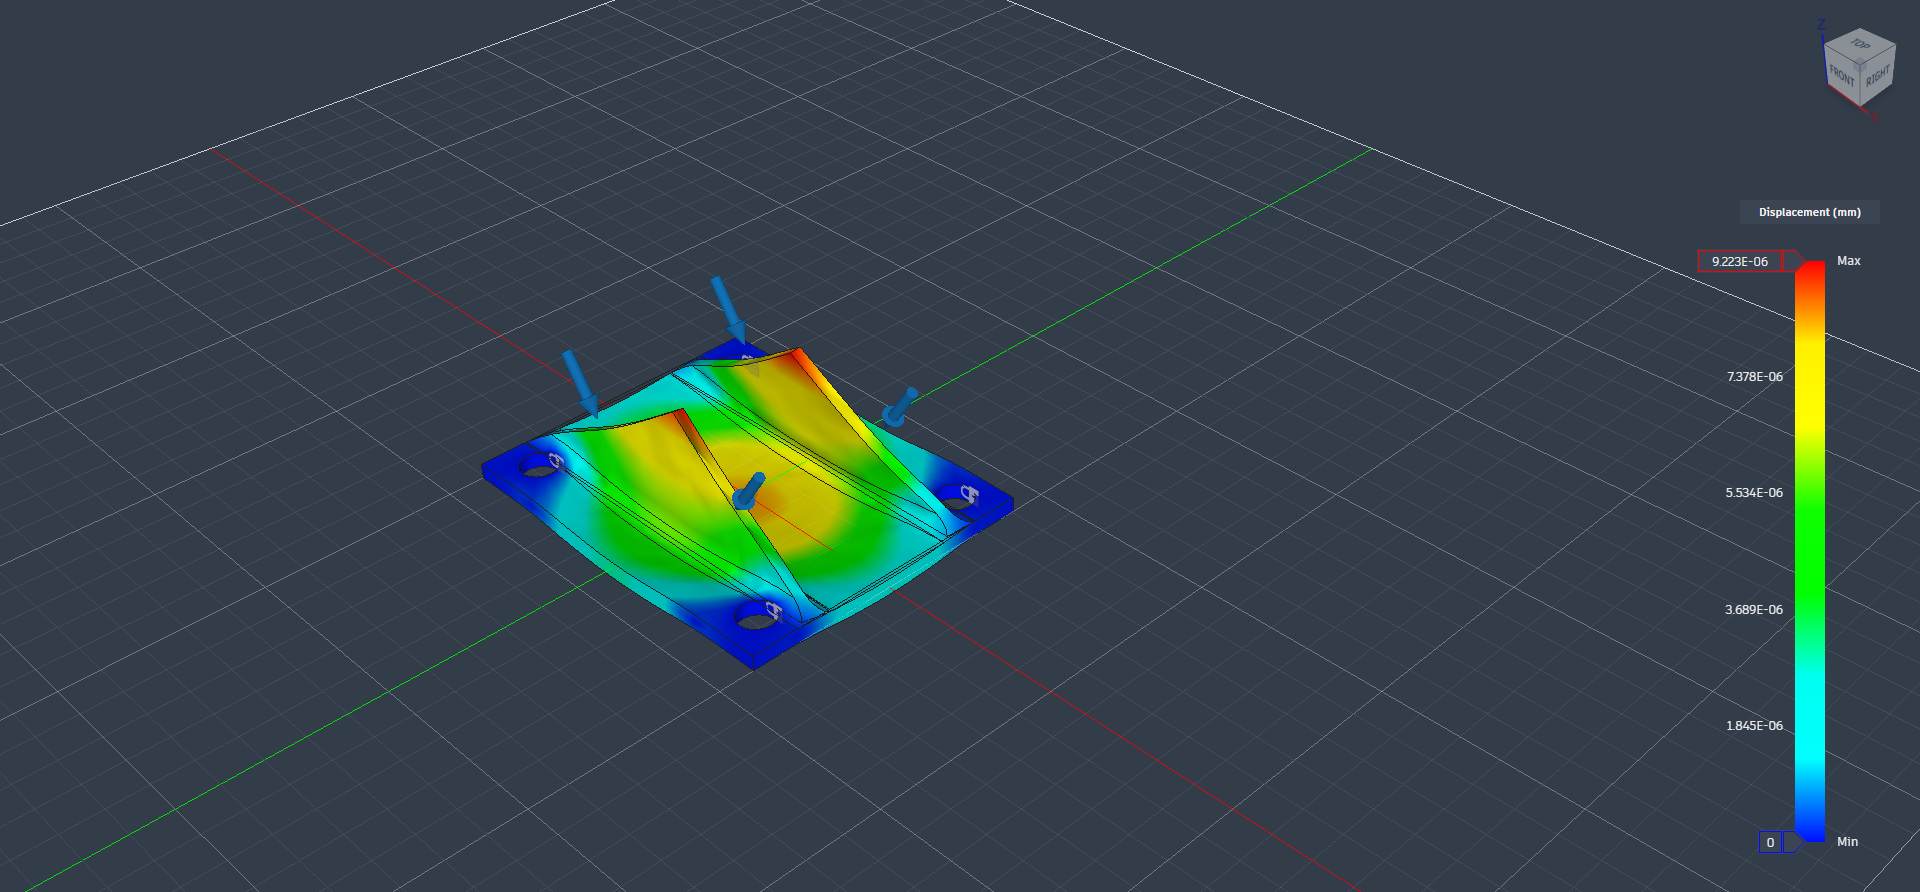
\includegraphics[width=\textwidth]{./images/fusion/study_2_09.png}
\caption*{(b) Study~2 total displacement}
\end{minipage}
\caption{Total-displacement distributions from Studies~1 and~2. The spatial
patterns are informative, but the magnitudes are invalid for the project load.}
\label{fig:bracket-displacement-comparison}
\end{figure}

The bracket studies therefore remain valuable as audit evidence. They confirm
that the native geometry reached the Simulation workspace, show the intended
support and load regions, and reveal plausible qualitative response
locations. They also demonstrate that solver completion is not an acceptance
criterion. A corrected 1472~N study must verify material data, direction,
reaction balance, contact assumptions, local mesh refinement, and convergence
before stress, factor of safety, or displacement is compared with the
analytical finalist.

\clearpage
\section{Discussion}
\label{sec:results-discussion}

\subsection{Achievement of the Project Objectives}
\label{sec:objective-achievement}

\begin{longtable}{
    >{\raggedright\arraybackslash}p{0.08\textwidth}
    >{\raggedright\arraybackslash}p{0.48\textwidth}
    >{\raggedright\arraybackslash}p{0.34\textwidth}}
\caption{Achievement of the specific objectives}
\label{tab:objective-achievement}\\
\toprule
\textbf{No.} & \textbf{Objective outcome} & \textbf{Status}\\
\midrule
\endfirsthead
\toprule
\textbf{No.} & \textbf{Objective outcome} & \textbf{Status}\\
\midrule
\endhead
\bottomrule
\endfoot
1 & Unit-aware parameter spaces, materials, loads, constraints, screening
models, and boundary roles were defined for all three components. &
Achieved for analytical screening and CAD preparation.\\
2 & Each part completed 60 seeded LHS evaluations and three bounded
Nelder--Mead starts; failed evaluations remained controlled. &
Achieved.\\
3 & Native Fusion geometry, physical properties, exchange artifacts, and
semantic boundary evidence were generated. &
Achieved for serialized CAD requests.\\
4 & Baseline plus 20-vector CAD sweeps and baseline/finalist validation sets
were completed. &
Achieved, with the stabilizer outer-process timeout disclosed.\\
5 & Lower-mass analytical finalists were selected and their mass estimates
were compared with native CAD. &
Achieved as screening evidence; all mass differences were within 3.8\%.\\
6 & The bracket proof of concept reached manual Static Stress review, and the
remaining evidence required for design acceptance was identified. &
Partly achieved; both exploratory solver studies were rejected and a corrected
1472~N study remains required.\\
\end{longtable}

\subsection{Limitations of the Results}
\label{sec:results-limitations}

The analytical models are intentionally first order. They use simplified load
paths, nominal section properties, and approximate concentration factors. The
reported constraints include yield-based factor of safety and displacement
only.

The search used a finite sample and three local starts. A different seed,
start, penalty, bound, or model can produce a different candidate. Several
finalists lie near lower bounds, so the selected bounds strongly influence the
result.

The CAD sweeps verify sampled geometry, not the full continuous design space.
They also do not check manufacturing drawings, tolerances, weld access, or
assembly.

The manual FEA evidence is incomplete. The available bracket report has an
incorrect load and cannot validate stress or displacement. Padeye and
stabilizer solver campaigns remain future work. No physical tests were
performed.

\subsection{Engineering Interpretation}

The results support the central workflow claim: inexpensive analytical
evaluation can reduce a large design set to a small group of traceable
candidates, and native CAD can check geometry and mass before manual FEA.
They do not support certification or fabrication.

The most important result is not the largest percentage reduction. It is the
separation of claims. The system recorded analytical predictions, returned
partial CAD responses without solver values, disclosed the stabilizer timeout,
and rejected a completed Fusion report after finding the wrong load. This
behavior is consistent with an auditable engineering workflow.
